\documentclass{standalone}
\usepackage{pgfplots}
\pgfplotsset{compat=1.17}
\usetikzlibrary{arrows.meta}


\colorlet{green_set}{green!70!black}
\colorlet{purple_set}{blue!80!cyan!60!red!95!black!90}
\colorlet{red_set}{red!80!black}
\colorlet{orange_set}{orange!80!}

\begin{document}
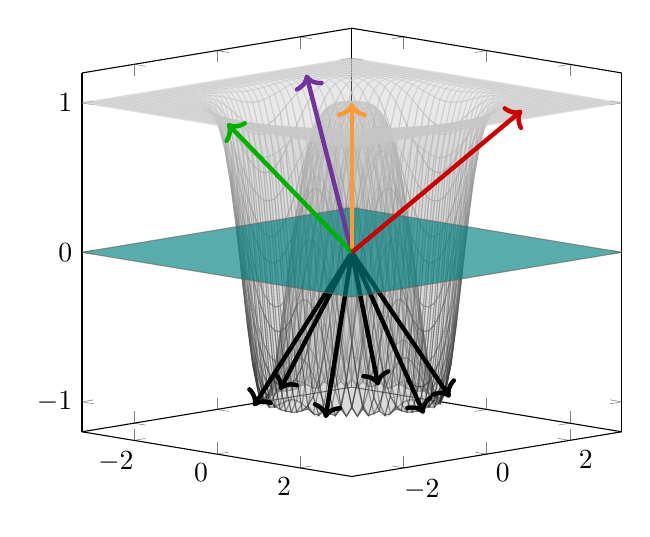
\begin{tikzpicture}
  \begin{axis}[
      view={45}{10},
      domain=-3.25:3.25,
      set layers,
      y domain=-3.25:3.25,
      samples=50,
      z buffer=sort,
      colormap={greyscale}{gray(0cm)=(0); gray(0.1cm)=(1)},
    ]
    \addplot3 [surf, 
      fill=lightgray,
    opacity=0.35] 
    {   1-((x^2 + y^2)^2/0.931194835465213) * e^(-(x^2 + y^2)^2/5.0625)
    };

    \draw[->, ultra thick, black] (axis cs:0,0,0) -- (axis cs:-0.866,-1.5,-1);
    \draw[->, ultra thick, black] (axis cs:0,0,0) -- (axis cs:0.866,-1.5,-1);

    \draw[->, ultra thick, black] (axis cs:0,0,0) -- (axis cs:-1.732,0,-1);
    \draw[->, ultra thick, black] (axis cs:0,0,0) -- (axis cs:1.732,0,-1);

    \draw[->, ultra thick, black] (axis cs:0,0,0) -- (axis cs:-0.866,1.5,-1);
    \draw[->, ultra thick, black] (axis cs:0,0,0) -- (axis cs:0.866,1.5,-1);

    \addplot3 [
      surf,
      fill=teal, 
      samples=2,
      opacity=0.65,
    ] 
    {0};

    \draw[->, ultra thick, purple_set] (axis cs:0,0,0) -- (axis cs:-2.598,1.5,1);
    \draw[->, ultra thick, orange_set] (axis cs:0,0,0) -- (axis cs:0,0,1);
    \draw[->, ultra thick, green_set] (axis cs:0,0,0) -- (axis cs:0,-3,1);
    \draw[->, ultra thick, red_set] (axis cs:0,0,0) -- (axis cs:2.598,1.5,1);

  \end{axis}
\end{tikzpicture}
\end{document}